
The subject of memory management in C++ can merit a book all of its own. There are dozens if not hundreds of papers dedicated just to the issue of the STL allocators. In this chapter, we will focus on several problems that tend to affect performance the most. Some have simple solutions; for others, we will describe the issue and outline the possible solution approaches. 

There are two types of memory-related problems that you may run into in the context of performance. The first one is using too much memory: your program either runs out of memory or doesn’t meet the memory use requirements. The second problem occurs when your program becomes memory-bound: its performance is limited by the speed of memory access. Often, in these cases, the runtime of the program is directly related to how much memory it uses, and reducing the memory use also makes the program run 
faster. 

The material presented in this section is helpful mostly for programmers who deal with memory-bound programs or programs that allocate memory frequently and/or in large quantities. We begin with the performance impact of the memory allocations themselves.

\subsubsubsection{9.4.1\hspace{0.2cm}Unnecessary memory allocations}

One of the most common performance problems related to memory use is that of unnecessary memory allocation. Here is a very common problem, described in C++-like pseudocode:

\begin{lstlisting}[style=styleCXX]
for ( … many iterations … ) {
	T* buffer = allocate(… size …);
	do_work(buffer); // Computations use memory
	deallocate(buffer);
}
\end{lstlisting}

A well-written program would use an RAII class to manage deallocations, but we wanted to make allocations and deallocations explicit for clarity. The allocations are usually concealed inside objects that manage their own memory, such as STL containers. It is not uncommon for such a program to spend most of its time in memory allocation and deallocation functions (such as malloc() and free()). 

We can see the effect on performance on a very simple benchmark:

\hspace*{\fill} \\ %插入空行
\noindent
\textbf{04\_buffer.C}
\begin{lstlisting}[style=styleCXX]
void BM_make_str_new(benchmark::State & state) {
	const size_t NMax = state.range(0);
	for (auto _: state) {
		const size_t N = (random_number() % NMax) + 1;
		char * buf = new char[N];
		memset(buf, 0xab, N);
		delete[] buf;
	}
	state.SetItemsProcessed(state.iterations());
}
\end{lstlisting}

Here the work is represented by initializing a character string, and the random\_number() function returns random integer values (it could be just rand(), but the benchmark is cleaner if we precompute and store random numbers to avoid benchmarking the random number generator). You may also need to trick thecompiler into not optimizing away the results: if the usual benchmark::DoNotOptimize()does not suffice, you may have to insert a print statement with the condition that never happens (but the compiler does not know it) like rand() < 0.

The numbers we get from the benchmark are meaningless by themselves: we need to compare them with something. In our case, the baseline is easy to figure out: we must do the same work but none of the allocations. This can be accomplished by moving the allocation and the deallocation out of the loop since we know the maximum memory size:

\hspace*{\fill} \\ %插入空行
\noindent
\textbf{04\_buffer.C}
\begin{lstlisting}[style=styleCXX]
char * buf = new char[NMax];
for (auto _: state) {
	…}
delete[] buf;
\end{lstlisting}

The performance difference you will observe in such a benchmark depends greatly on the operating system and the system libraries, but you’re likely to see something like this (we used strings of random sizes up to 1 KB):

\hspace*{\fill} \\ %插入空行
\begin{center}
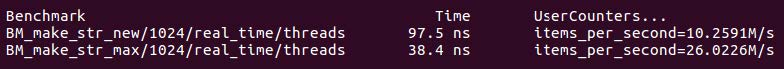
\includegraphics[width=0.9\textwidth]{content/3/chapter9/images/5.jpg}\\
Figure 9.5 – Performance impact of the allocation-deallocation pattern
\end{center}

It should be noted that the memory allocations in a micro-benchmark are typically more efficient than in the context of a large program where the memory allocation pattern is much more complex, so the real-world effect of frequent allocations and deallocations is likely to be even larger. Even in our small benchmark, the implementation that allocates memory every time runs at 40\% of the speed of the version that allocates the maximum possible amount of memory just once. 

Of course, when the maximum amount of the memory we need during the computation is known in advance, preallocating it and reusing it from one iteration to the next is an easy solution. This solution generalizes to many containers as well: for a vector or deque, we can reserve the memory before the start of the iterations and take advantage of the fact that resizing the container does not shrink its capacity.

The solution is only slightly more complex when we do not know the maximum memory size in advance. This situation can be handled with a grow-only buffer. Here is a simple buffer that can be grown but never shrinks:

\hspace*{\fill} \\ %插入空行
\noindent
\textbf{04\_buffer.C}
\begin{lstlisting}[style=styleCXX]
class Buffer {
	size_t size_;
	  std::unique_ptr<char[]> buf_;
	public:
	explicit Buffer(size_t N) : size_(N), buf_(
	new char[N]) {}
	void resize(size_t N) { 
		if (N <= size_) return;
		char* new_buf = new char[N];
		memcpy(new_buf, get(), size_);
		buf_.reset(new_buf);
		size_ = N;
	}
	char* get() { return &buf_[0]; }
};
\end{lstlisting}

Again, this code is useful for demonstration and exploration. In a real program, you are likely to use STL containers or your own library classes, but they all should have the capability to increase the memory capacity. We can compare the performance of this grow-only buffer with that of the fixed-size preallocated buffer by trivially modifying our benchmark:

\hspace*{\fill} \\ %插入空行
\noindent
\textbf{04\_buffer.C}
\begin{lstlisting}[style=styleCXX]
void BM_make_str_buf(benchmark::State& state) {
	const size_t NMax = state.range(0);
	Buffer buf(1);
	for (auto _ : state) {
		const size_t N = (random_number() % NMax) + 1;     
		buf.resize(N);
		memset(buf.get(), 0xab, N);
	}
	state.SetItemsProcessed(state.iterations());
}
\end{lstlisting}

Again, in a real program, you are likely to get better results with a smarter memory growth strategy (grow by somewhat more than requested, so you don’t have to grow memory as often – most STL containers employ some form of this strategy). But, for our demonstration, we want to keep things as simple as possible. On the same machine, the results of the benchmark are as follows:

\hspace*{\fill} \\ %插入空行
\begin{center}
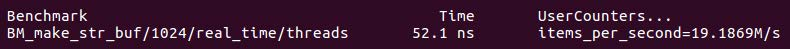
\includegraphics[width=0.9\textwidth]{content/3/chapter9/images/6.jpg}\\
Figure 9.6 – Performance of a grow-only buffer (compare with Figure 9.5)
\end{center}

The grow-only buffer is slower than a fixed-size buffer but much faster than allocating and deallocating memory every time. Again, a better growth policy would make this buffer even faster, close to the speed of the fixed-size buffer. 

This is not the entire story: the importance of good memory management is even greater in multi-threaded programs because the calls to the system memory allocator do not scale well and may involve a global lock. Running our benchmark on the same machine using 8 threads produces these results:

\hspace*{\fill} \\ %插入空行
\begin{center}
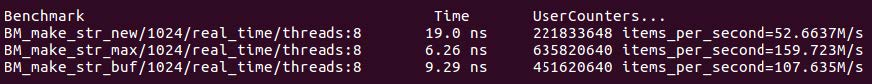
\includegraphics[width=0.9\textwidth]{content/3/chapter9/images/7.jpg}\\
Figure 9.7 – Performance impact of the allocation-deallocation pattern in a multi-threaded program
\end{center}

Here, the penalty for frequent allocations is even greater (the grow-only buffer shows the cost of the remaining allocations as well and would really benefit from a smarter growth policy). 

The bottom line is: interact with the OS as little as possible. If you have a loop that needs to allocate and deallocate memory on each iteration, allocate once before the loop instead. If the allocations are of the same size, or you know the maximum allocation size upfront, make one allocation of this size and hold it (of course, if you use several buffers or containers, you should not try to shoehorn them into a single allocation, but preallocate each one). If you do not know the maximum size, use a data structure that can grow, but do not shrink or release the memory until the work is done. 

The recommendation to avoid interacting with the OS is particularly important in multi-threaded programs, and we will now make some more general comments on the use of memory in concurrent programs.

\subsubsubsection{9.4.2\hspace{0.2cm}Memory management in concurrent programs}

The memory allocator provided by the operating system is a solution that balances many requirements: on a given machine, there is only one OS but many different programs with their own unique needs and memory use patterns. The developers tried very hard to make it not fail miserably in any reasonable use case; the flip side is that it’s rarely the best possible solution for any use case, too. Often, it’s good enough, especially if you follow the recommendation of requesting memory frequently.

Memory allocation becomes more inefficient in concurrent programs. The primary reason is that any memory allocator has to maintain a fairly complex internal data structure to track allocated and free memory. In high-performance allocators, the memory is subdivided into multiple arenas to group allocations of similar size together. This increases performance at the cost of complexity. The result is that this management of the internal data has to be protected by a lock if multiple threads are allocating and deallocating memory at once. This is a global lock, one for the entire program, and it can limit the scaling of the entire program if the allocator is called often.

The most common solution to this problem is to use an allocator with thread-local caches, such as the popular malloc() replacement library TCMalloc. These allocators reserve some amount of memory for each thread: when a thread needs to allocate memory, it is taken from the thread-local memory arena first. This does not need a lock since only one thread interacts with that arena. Only if the arena is empty does the allocator have to take the lock and allocate from the memory shared between all threads. Similarly, when a thread deallocates the memory, it is added to the thread-specific arena, again without any locking.

The thread-local caches are not without their share of problems.

First of all, they tend to use more memory overall: if one thread frees a lot of memory and another thread allocates a lot of memory, the recently freed memory does not become available to the other thread (it’s local to the thread that released it). So more memory is allocated while unused memory is available for other threads. To limit this memory waste, he allocators typically do not allow the per-thread arena to grow above some predefined limit. Once the limit is reached, the thread-local memory is returned to the main arena shared between all threads (this operation requires a lock).

The second problem is that these allocators work well if each allocation is owned by one thread, that is, the same thread allocates and deallocates memory at each address. If one thread allocates some memory, but another thread has to deallocate it, this cross-thread deallocation is difficult because the memory must be transferred from the thread-local arena of one thread to that of the other (or to the shared arena). A simple benchmark shows that the performance of cross-thread deallocation with the standard allocators like malloc() or TCMalloc is at least an order of magnitude worse than that of thread-owned memory. This is likely to be true with any allocator that utilizes thread-local caches, and so memory transfers between threads should be avoided whenever possible.

So far, we were talking about transferring memory from one thread to another for the purpose of deallocating it. What about simply using memory that was allocated by another thread? The performance of such memory access depends greatly on the hardware capabilities. For a simple system with few CPUs, this is likely a non-issue. But larger systems have multiple memory banks, and the connection between the CPU and the memory is not symmetric: each memory bank is closer to one CPU. This is known as the non-uniform memory architecture (NUMA). The performance impact of NUMA varies widely from doesn’t matter to twice as fast. There are ways to tune theperformance of the NUMA memory system as well as making the program memory management sensitive to NUMA details, but beware that you are likely tuning the performance to a particular machine: there is very little that can be said about the performance of NUMA systems in general.

We are now returning to the issue of using memory more efficiently since it is universally helpful for performance in concurrent and serial programs alike.


\subsubsubsection{9.4.3\hspace{0.2cm}Avoiding memory fragmentation}

One issue that plagues many programs is an inefficient interaction with the memory allocation system. Let us say that the program needs to allocate 1 KB of memory. This chunk of memory is carved out from some larger memory arena, marked as used by the allocator, and the address is returned to the caller. More memory allocations follow, so the memory after our 1 KB chunk is now used too. Then the program returns the first allocation and immediately asks for 2 KB of memory. There is a 1 KB free chunk, but it’s not large enough to service this new request. There may be another 1 KB chunk somewhere else, but as long as the two chunks are not right next to each other, they are not useful for the purpose of the 2 KB allocation:

\hspace*{\fill} \\ %插入空行
\begin{center}
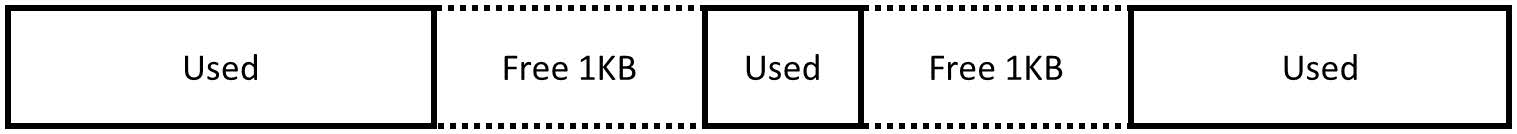
\includegraphics[width=0.9\textwidth]{content/3/chapter9/images/8.jpg}\\
Figure 9.8 – Memory fragmentation: 2 KB of free memory exists but is not useful for a single 2 KB allocation
\end{center}

This situation is known as memory fragmentation: the system has free memory returned by the program but instead has to use new memory to service the next allocation because the memory released by the program is fragmented into small chunks. In extreme cases, this fragmentation can cause the program to run out of memory long before the overall memory capacity of the system is exhausted (the worst case the author has seen is a program that ran out of memory after allocating only 1/6th of the total memory available). There are memory allocators that resist fragmentation better than the standard malloc(), but for programs that churn through memory quickly, more extreme measures may be required.

One such measure is a block allocator. The idea is that all memory is allocated in blocks of fixed size, such as 64 KB. You should not allocate single blocks of this size from the OS one at a time but instead allocate larger chunks of fixed size (say, 8 MB) and subdivide them into the smaller blocks (64 KB in our example). The memory allocator that handles these requests is the primary allocator in your program, the one that interacts directly with malloc(). Because it allocates blocks of just one size, it can be very simple, and we can focus on the most efficient implementation (thread-local cache for concurrent programs, low latency for real-time systems, and so on). Of course, you do not want to deal with these 64 KB blocks everywhere in your code. That is the job of secondary allocators, as shown in the following Figure 9.9:

\hspace*{\fill} \\ %插入空行
\begin{center}
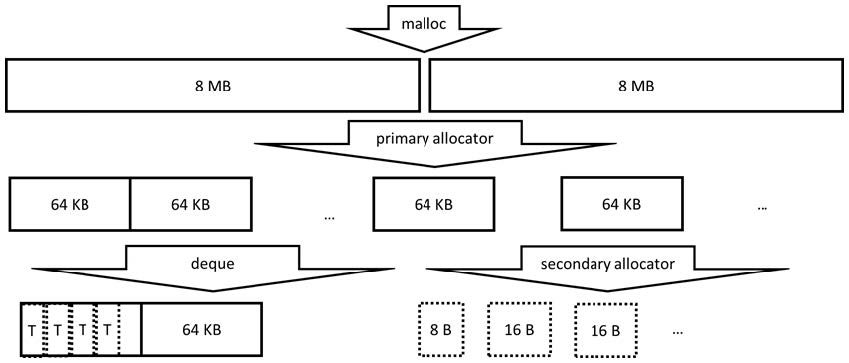
\includegraphics[width=0.9\textwidth]{content/3/chapter9/images/9.jpg}\\
Figure 9.9 – Fixed-size block allocation
\end{center}

You can have an allocator that further subdivides the 64 KB blocks into smaller allocations. Particularly efficient is a uniform allocator (an allocator for just one size): for example, if you want to allocate memory for single 64-bit integers, you can do so without any memory overhead (by comparison, malloc() usually requires at least 16 bytes of overhead per allocation). You can also have containers that allocate memory in 64 KB blocks and use it to store the elements. You will not be using vectors since they require a single large, contiguous allocation. The array-like container you want here is the deque that allocates memory in fixed-size blocks. You can, of course, have nodal containers as well. You can use the STL containers if the STL allocator interface is sufficient for your needs; otherwise, you may have to write your own container library.

The key advantage of the fixed-size block allocation is that it does not suffer from fragmentation: all allocations from malloc() are of the same size, so are all allocations from the primary allocator. Any time a memory block is returned to the allocator, it can be reused to satisfy the next request for memory. Refer to the following figure:

\hspace*{\fill} \\ %插入空行
\begin{center}
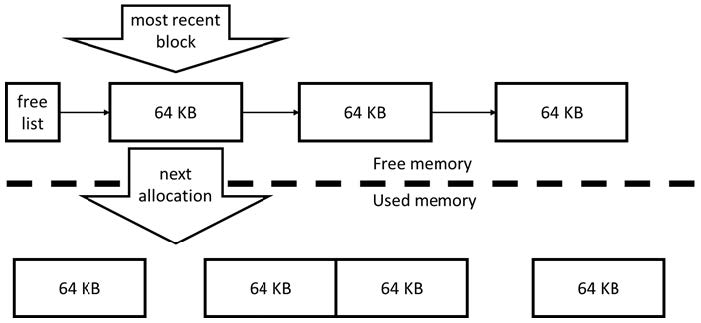
\includegraphics[width=0.9\textwidth]{content/3/chapter9/images/10.jpg}\\
Figure 9.10 – Memory reuse in fixed-size allocators
\end{center}

That first-in-first-out property is also an advantage: the last 64 KB memory block is likely to be from the most recently used memory and is still hot in the cache. Reusing this block immediately improves memory reference locality and, therefore, makes more efficient use of the cache. The allocator manages the blocks returned to it as a simple free list (Figure 9.10). These free lists can be maintained per thread to avoid locking, although they will likely need periodic rebalancing to avoid the situation where one thread has accumulated many free blocks while another thread is allocating new memory.

Of course, the allocators that subdivide our 64 KB blocks into smaller sizes are still susceptible to fragmentation unless they are also uniform (fixed-size) allocators. It is, however, easier to write a self-defragmenting allocator if it has to deal with a small memory range (one block) and few different sizes. 

It is likely that the entire program is affected by the decision to use block memory allocation. For example, allocating large numbers of small data structures such that each one uses a fraction of the 64 KB block and leaves the rest unused becomes prohibitively expensive. On the other hand, a data structure that itself is a collection of smaller data structures (a container) such that it packs many smaller objects into one block becomes easier to write. One can even write compressed containers that compress each block for keeping the data long-term, then decompress them one block at a time for access. 

The block size itself is not set in stone, either. Some applications will be more efficient with smaller blocks where less memory is wasted if a block is left partially unused. Others can benefit from larger blocks that require fewer allocations.

The literature on application-specific allocators is extensive. For example, slab allocators are a generalization of the block allocators we have just seen; they manage multiple allocation sizes efficiently. There are many other types of custom memory allocators, and most of them can be used in a C++ program. Using an allocator that is well-suited for a specific application often brings dramatic performance improvements, usually at the cost of severely restricting the programmer’s freedom in the implementation of the data structures.

The next common reason for inefficiency is more subtle and much harder to deal with.





















